% !TEX TS-program = pdflatex
% !BIB TS-program = biber
\documentclass[12pt,letterpaper]{article}

% Layout and formatting
\usepackage[margin=1in]{geometry}
\usepackage{acronym}
\usepackage{csquotes}
\usepackage{fixltx2e}
\usepackage{url}
\usepackage[T1]{fontenc}
\usepackage{mathptmx}
\usepackage{setspace}
\usepackage{units}
\usepackage{etoolbox}
\BeforeBeginEnvironment{equation}{\begin{singlespace}}
\AfterEndEnvironment{equation}{\end{singlespace}\noindent\ignorespaces}
\BeforeBeginEnvironment{align}{\begin{singlespace}}
\AfterEndEnvironment{align}{\end{singlespace}\noindent\ignorespaces}
\frenchspacing

% Graphics
\usepackage{graphicx}
\usepackage[pdf]{pstricks}
\psset{unit=1in,linewidth=0.02,arrows=C-C,arrowsize=0.2}

% Bibliography
\usepackage[american]{babel}
\usepackage[backend=biber,style=apa]{biblatex}
\DeclareLanguageMapping{american}{american-apa}
\bibliography{bibliography.bib}
\newcommand{\aposcite}[2]{\citeauthor{#1}'s #2 (\citeyear{#1})}
\usepackage{doi}

% Figures, tables, and captions
\usepackage{float}
\usepackage{booktabs}
\usepackage[hypcap]{caption}
\captionsetup{labelfont=bf,font=small,labelsep=period}
\usepackage{subcaption}
\usepackage[rightcaption]{sidecap}
\usepackage[plain]{fancyref}

% Math
\usepackage{amsmath}
\usepackage[algoruled]{algorithm2e}
\usepackage{mathtools}
\usepackage{commath}

\title{Bayesian Reconstruction of Coevolutionary Histories}

% Acronyms
\acrodef{GMTC}{geographic mosaic theory of coevolution}
\acrodef{GTR}{general time reversible}
\acrodef{MCMC}{Markov chain Monte Carlo}
\acrodef{ESS}{estimated sample size}
\acrodef{MCC}{maximum clade credibility}

% Reusable figures
\newcommand{\pscophylogeny}{
\begin{pspicture}(18,12)
\psset{unit=0.5cm,linewidth=0.2}
\psline[linecolor=blue](0,0)(10,10)
\psline[linecolor=blue](4,0)(2,2)
\psline[linecolor=blue](8,0)(4,4)
\psline[linecolor=blue](12,0)(14,2)
\psline[linecolor=blue](16,0)(8,8)
\psline[linecolor=red](1,0)(11,10)
\psline[linecolor=red,arrows=-o](17,0)(9,8)
\psline[linecolor=red,arrows=-o](13,0)(15,2)
\psline[linecolor=red](7,3)(14,3)
\psline[linecolor=red,arrows=<-](10,3)(14,3)
\psline[linecolor=red](10,0)(7,3)
\psline[linecolor=red,arrows=-o](9,0)(5,4)
\psline[linecolor=red,arrows=-o](4,1)(3,2)
\rput{135}(4,1){\LARGE\textcolor{red}{\textsf{\textbf{x}}}}
\psline[linecolor=red](18,0)(17,1)
\psline[linecolor=red,arrows=*-](16,1)(17,1)
\end{pspicture}
}

\begin{document}

\begin{titlepage}
\null
\vfil
\let\newpage\relax
\maketitle
\vfil
\centering
\pscophylogeny
\vfil
\thispagestyle{empty}
\end{titlepage}

\newpage

\doublespacing

\section*{Introduction}

Organismic symbioses, or interactions between individuals of two or more different species, constitute a fundamental aspect of many living systems and occur across the biological spectrum. The characteristics of symbiotic relationships can vary greatly, particularly in degrees of cooperation (parasitism vs. mutualism), fidelity (generalized vs. specialized and species-specific), and obligation (optional vs. vital to survival) \parencites{Herre:1999}{Charleston:2002}{Oberprieler:2004}{Machado:2005}{Becerra:2007}{Beinart:2012}{HoyalCuthill:2012}{Thompson:2012}{Faria:2013}. Understanding how these relationships evolve and, in particular, how symbionts affect their partners' evolution---that is, the coevolutionary processes driven by symbiotic interactions---remain important questions in ecology and evolutionary biology. 

Phylogenies, or evolutionary trees, can provide a valuable perspective to evolutionary processes. The topology of a phylogenetic tree depicts the series of speciation events that gave rise to a set of taxa and thus their ancestral relationships \parencite{Baum:2008}. Often, the lengths of branches indicate the number of substitutions (e.g., genetic mutations) accumulated or the amount of time passed at that particular lineage \parencite{Baum:2008}. By mapping traits such as physical attributes or geographic locations onto a known phylogeny, we can use the tree to learn about the mechanisms under which these traits change \parencites{Lemey:2009}{Lemey:2010}{Segraves:2010}.

Molecular sequences are the primary source of data for constructing phylogenies \parencite{Baum:2008}. With the advancements of DNA sequencing technology over the last few decades, considerable effort has been invested in developing robust statistical methods for inferring phylogenies from sequence alignments (of both nucleotides and amino acids) \parencite{Felsenstein:2005}. One of the first techniques for phylogenetic inference optimized the tree topology under the parsimony criterion \parencite{Fitch:1971}. The most parsimonious tree is the \enquote{simplest} possible explanation for the  sequence alignment: the tree involving the least number of substitution events. Following his criticism of parsimony methods \parencite{Felsenstein:1978}, \textcite{Felsenstein:1981} introduced an algorithm to calculate the likelihood of a tree given a sequence alignment and a substitution model. Similar to maximum parsimony, maximum likelihood techniques optimize a tree under \aposcite{Felsenstein:1981}{likelihood function}, often simultaneously estimating parameter values for the substitution model \parencite{Felsenstein:2005}. Likelihood methods can be used with sophisticated substitution models, such as models that consider the underlying molecular processes of evolution \parencite[e.g.,][]{Hasegawa:1985}.

Many recent advances in phylogenetics have focused on methodologies utilizing Bayesian inference \parencites{Ronquist:2012}{Drummond:2012}. Bayesian inference takes its name from Bayes' theorem \parencite{Bayes:1763} and relies on the principle that the posterior probability of a model's parameters~$\theta$ given some unchanging data~$D$ is $P\left(\theta|D\right) \propto P\left(D|\theta\right) P\left(\theta\right)$. The likelihood, $P\left(D|\theta\right)$, is the probability of simulating the observed data under the model parameters (e.g., \citeauthor{Felsenstein:1981}'s \citeyear{Felsenstein:1981} algorithm), and the prior, $P\left(\theta\right)$, is the probability of the model parameters without considering the data. The prior can be a mechanism to apply previous knowledge to a new analysis; for example, constructing a prior distribution on the mutation rate parameter that is representative of the rates reported in previous literature will \enquote{bias} the posterior to favor those rates. When explicit prior knowledge is not available, an uninformative prior may be applied.

Often we are interested in only some of the parameters involved in an analysis (e.g., just the tree topology), in which case we can calculate the posterior probability of specific values for those parameters by integrating over all possible values of the remaining \enquote{nuisance} parameters (branch lengths, mutation rate, etc.). Due to the complexity of the models, the resulting multi-dimensional integral cannot be evaluated directly but instead approximated via a \ac{MCMC}. Under the Metropolis--Hastings \ac{MCMC} algorithm, the chain advances from one state, or set of parameter values, to the next by randomly mutating the current state and accepting or rejecting this proposal based on its posterior probability \parencites{Metropolis:1953}{Hastings:1970}. With a chain of enough length, the collection of states sampled by the \ac{MCMC} is an approximation of the posterior distribution. Although there have been criticisms of Bayesian \ac{MCMC} methodologies in phylogenetics \parencites{Felsenstein:2005}{Kolaczkowski:2009}, they remain popular for their flexibility, particularly the ability to adopt complex evolutionary models and integrate over uncertainties \parencites{Huelsenbeck:2000}{Drummond:2007}{Ronquist:2012}.

\textcite{Haffner:1988} were the first to apply phylogenetic methods to study coevolution. After constructing phylogenies for pocket gophers and their parasitic lice, they presented them side-by-side for comparison. Although the speciation patterns between the two trees showed significant similarities, they were not identical, which leads to an important observation: that host--symbiont phylogenies generally do not mirror each other perfectly, even in highly-specialized, obligatory mutualisms \parencite{Machado:2005}. Therefore, there must be other processes involved

It is important to note that the host--symbiont cophylogeny reconstruction problem is very similar to the gene tree--species tree reconciliation problem involving horizontal gene transfers. As with host and symbiont phylogenies, phylogenies of individual genes often do not correspond with the phylogeny of the species themselves \parencite{Heled:2010a}, especially in the case of bacteria, which can transfer genetic material between species (horizontal gene transfer) \parencite{David:2011}.



There are generally (\Fref{fig:events})

\begin{figure}
\centering
\begin{subfigure}[b]{0.2\textwidth}
\centering
\begin{pspicture}(1,1)
\psline[linecolor=blue](0,0.5)(0.5,0.5)
\psline[linecolor=blue](0.5,0.3)(1,0.3)
\psline[linecolor=blue](0.5,0.7)(1,0.7)
\psline[linecolor=blue](0.5,0.3)(0.5,0.7)
\psline[linecolor=red](0.4,0.4)(1,0.4)
\psline[linecolor=red](0.4,0.8)(1,0.8)
\psline[linecolor=red](0.4,0.4)(0.4,0.8)
\psline[linecolor=red,arrows=-o](0,0.6)(0.4,0.6)
\end{pspicture}
\caption{cospeciation}
\end{subfigure}
\begin{subfigure}[b]{0.2\textwidth}
\centering
\begin{pspicture}(1,1)
\psline[linecolor=blue](0,0)(1,0)
\psline[linecolor=red](0,0.1)(1,0.1)
\psline[linecolor=red,arrows=*-](0.5,0.1)(0.5,0.3)
\psline[linecolor=red](0.5,0.3)(1,0.3)
\end{pspicture}
\caption{duplication}
\end{subfigure}
\begin{subfigure}[b]{0.2\textwidth}
\centering
\begin{pspicture}(1,1)
\psline[linecolor=blue](0,0)(1,0)
\psline[linecolor=blue](0,0.4)(1,0.4)
\psline[linecolor=red](0,0.1)(1,0.1)
\psline[linecolor=red](0.5,0.1)(0.5,0.5)
\psline[linecolor=red,arrows=->,arrowsize=0.1](0.5,0.1)(0.5,0.35)
\psline[linecolor=red](0.5,0.5)(1,0.5)
\end{pspicture}
\caption{host-switch}
\end{subfigure}
\begin{subfigure}[b]{0.2\textwidth}
\centering
\begin{pspicture}(1,1)
\psline[linecolor=blue](0,0)(1,0)
\psline[linecolor=red](0,0.1)(0.8,0.1)
\rput(0.8,0.1){\large\textcolor{red}{\textsf{x}}}
\end{pspicture}
\caption{loss}
\end{subfigure}
\caption{Diagrams of the four cophylogenetic events considered in my model, where the host organism's phylogeny is in blue and the symbiont phylogeny in red. All events are branch events (i.e., they can occur at any point along a branch) except cospeciation, which is a nodal event (and thus can occur only when the host speciates).}
\label{fig:events}
\end{figure}

There are a number of programs implementing event-based models for maximum parsimony reconstruction of , e.g., Tarzan \parencite{Merkle:2005}, CoRe-PA \parencite{Merkle:2010}, Jane \parencite{Conow:2010}, TreeMap \parencite{Charleston:2011}, and AnGST \parencite{David:2011}.

Brooks Parsimony Analysis \parencite{Brooks:1981} and the coalescent \parencite{Rannala:2003} were also proposed as methods  

However, the cophylogeny reconstruction problem could benefit from a probabilistic approach .

The fundamental challenge  \parencite{Charleston:2009}: at any point in time, a symbiont may have duplicated on its host or switched to another host . ; a closed-form solution exists only for the simpler duplication-loss problem \parencite{Gernhard:2008} which does not consider host-shift/transfer events.

 \textcite{Huelsenbeck:2000} presented the first such solution, a Bayesian \ac{MCMC} implementation of a simple model that considered only host-switch events; however, it was not developed further.

More recently, \textcite{Charleston:2009} described a complex model and proposed that discretization be used to approximate

. , in the context of the gene tree--species tree problem.


\textcite{Faria:2013} ; however, they treat the host phylogeny as fixed and develop a specific rate matrix to describe a transition of the symbiont from any 


A Bayesian \ac{MCMC} method for inferring cophylogenies also lends a number of advantages.

A primary objective of parsimony approaches to the cophylogeny problem is developing heuristics to find optimal reconstructions quickly. For example, \textcite{Charleston:1998} proposed the \enquote{jungle} concept and the program Jane utilizes a genetic algorithm to find optimal timings \parencite{Conow:2010} . This problem becomes much less of a concern in an \ac{MCMC} framework, because the parameter space is being explored as opposed to maximized (although it is still critical to employ effective operators for efficient mixing of the chain). However, it is important to note that \ac{MCMC} methods carry a much greater computational expense. 

I describe a simple cophylogeny model to approximate the likelihood of a cophylogenetic reconstruction and implement it in a Bayesian framework. To evaluate my algorithm, I run analyses on data simulated under the model.

\begin{SCfigure}
\centering
\pscophylogeny
\caption{An example of a coevolutionary history, with the host phylogeny in blue, the symbiont phylogeny in red, and symbols corresponding with the four events depicted in \Fref{fig:events}.}
\label{fig:cophylogeny}
\end{SCfigure}

\section*{Materials and Methods}

Given data~$D = \left(d_H,d_S,d_R\right)$, the host sequence data, the symbiont sequence data, and the leaf--leaf associations between the host and symbiont trees, respectively, I define the posterior probability of the host tree~$H$ and the symbiont tree~$S$, both with branch lengths, and the reconstruction~$R$ mapping internal nodes of $S$ to $H$ as
\begin{equation}
P\left(H,S,R|D\right) \propto \int P\left(d_S\right|S) P\left(S|H,R,d_R,\theta\right) P\left(H|d_H\right) P\left(R\right) P\left(\theta\right) \, \dif \theta
\label{eq:cophylogenyposterior}
\end{equation}
where parameters $\theta = \left(\lambda,\tau,\mu\right)$, the duplication, host-switch, and loss rates, respectively, and are integrated out. The probability of a tree~$T$ given sequence data~$D$ is $P\left(T|D\right) \propto P\left(D|T\right) P\left(T\right)$, where the likelihood is generally calculated with \aposcite{Felsenstein:1981}{algorithm} or a more complex multi-locus model, e.g. the multispecies coalescent \parencite{Heled:2010a}, and the prior with either a coalescent model \parencite{Kingman:1982} or a birth-death speciation model \parencite{Gernhard:2008}. In this case, the prior on the symbiont tree is represented instead by the reconstruction likelihood $P\left(S|H,R,d_R,\theta\right)$.

The key term is $P\left(S|H,R,d_R,\theta\right)$, the likelihood of the cophylogenetic reconstruction, and it is equivalent to a summation over the reconstruction likelihoods for all theoretical symbiont phylogenies and reconstructions of which we can only observe $S$ and $d_R$ (due to extinction events, etc.). Because we cannot calculate this term analytically, I approximate the likelihood of a reconstruction by treating the event rates $\theta$ as rates of observation (vs. the actual rates of occurrence). It is possible to enumerate a set of potential cases, in each where a specific series of events is observed.

\paragraph*{Determining the events.}

The symbiont phylogeny $S$ and the host phylogeny $H$ are represented as rooted, bifurcating trees. I refer to the nodes, or vertices, of a tree T as $V(T)$, where the leaves $L(T) = \{v : v \in V(T) \wedge \deg^+(v)=0\}$, the internal nodes $I(T) = V(T) \setminus I(T)$, and the root $root(T)$ has $\deg^-(root(T)) = 0$. The two children of an internal node are represented by $\text{left}(v)$ and $\text{right}(v)$, and its parent by $parent(v)$, granted that it is not the root ($deg^-(v)>0$). The height of a node from the tips is $height(v)$ and the length of its branch $(v, parent(v))$ is $l(v)$, both in units of time.

\begin{SCfigure}[1.5]
\centering
\begin{pspicture}(18,12)
\psset{unit=0.25cm,linewidth=0.3}
\psline(0,0)(10,10)
\psline(4,0)(2,2)
\psline(8,0)(4,4)
\psline(12,0)(14,2)
\psline(16,0)(8,8)
\rput(0,-0.75){\small\textbf{1}}
\rput(4,-0.75){\small\textbf{2}}
\rput(8,-0.75){\small\textbf{3}}
\rput(12,-0.75){\small\textbf{4}}
\rput(16,-0.75){\small\textbf{5}}
\rput(16,-0.75){\small\textbf{5}}
\rput(1.5,2.5){\small\textbf{6}}
\rput(3.5,4.5){\small\textbf{7}}
\rput(14.5,2.5){\small\textbf{8}}
\rput(7.5,8.5){\small\textbf{9}}
\end{pspicture}
\caption{In the depicted topology, node 6 is a \textsc{descendant} of nodes 7 and 9, an \textsc{ancestor} of nodes 1 and 2, and a \textsc{cousin} of all other nodes.}
\label{fig:nodalrelationships}
\end{SCfigure}

I define the topological relationship of node~$n \in V(T)$ relative to node~$r \in V(T)$ in tree~$T$ as

\begin{equation}
relationship(n, r) = 
\begin{cases}
\text{\textsc{self}}, & \text{if}\ n = r \\
\text{\textsc{descendant}}, & \text{if}\ r \in ancestors(n) \\
\text{\textsc{ancestor}}, & \text{if}\ n \in ancestors(r) \\
\text{\textsc{cousin}}, & \text{otherwise} \\
\end{cases}
\end{equation}
\doublespacing
where $ancestors(v)$ is defined as the set $A$ where, given that $\deg^-(v) > 0$, $parent(v) \in A$ and, if $u \in A$ and $\deg^-(u) > 0$, then $parent(u) \in A$. When $\deg^-(v) = 0$, $ancestors(v) = \emptyset$. An example is given in \Fref{fig:nodalrelationships}.

My model requires that a symbiont be contemporaneous with its host, such that for a node $s \in V(S)$, $height(host(s)) \leq height(s) < height(host(parent(s)))$, where the second condition may be dropped when $host(s)$ is the root. If this is satisfied, the likelihood at $s$ is given by Algorithm 1; otherwise, the likelihood of the reconstruction is considered to be $L=0$

\newcommand{\defcase}[2]{$r_\text{left} = \text{\textsc{#1}}$ and $r_\text{right} = \text{\textsc{#2}}$}

\begin{algorithm}
\caption{Probability of the reconstruction at a given node of the symbiont tree.}

\KwIn{$s \in I(S)$}

$duplication(t) := $ probability of duplication at time $t$\;
$hostswitch(t) := $ probability of host-switch at time $t$\;
$losses(s) := $ probability of any losses along $H$ incurred by $s \in V(S)$\;
$loss(t,l) := $ probability of a loss along lineage $l \in V(H)$ starting from time $t$\;
$noevent(t) := $ probability of no event by time $t$\;

$h_\text{self} := host(s)$, $h_\text{left} := host(\text{left}(s))$, $h_\text{right} := host(\text{right}(s))$\;

$r_\text{left} := relationship(h_\text{left},h_\text{self})$, $r_\text{right} := relationship(h_\text{right},h_\text{self})$\;

\uIf
(\tcp*[h]{see \Fref{fig:algoselfself}})
{\defcase{self}{self}}
{\tcp{duplication event}
\Return $duplication(l(s))$\;}
\uElseIf
(\tcp*[h]{see \Fref{fig:algoselfcousin}})
{\defcase{self}{cousin}}
{\tcp{host-switch event}
\Return $hostswitch(l(s)) \times losses(\text{right}(s))$\;}
\uElseIf
(\tcp*[h]{opposite child of previous case})
{\defcase{cousin}{self}}
{\Return $hostswitch(l(s)) \times losses(\text{left}(s))$\;}
\uElseIf
(\tcp*[h]{see \Fref{fig:algodescendantcousin}})
{\defcase{descendant}{cousin}}
{\tcp{host-switch event}
\Return $hostswitch(l(s)) \times losses(\text{left}(s)) \times losses(\text{right}(s)))$\;}
\uElseIf
(\tcp*[h]{opposite child})
{\defcase{cousin}{descendant}}
{\Return $hostswitch(l(s)) \times losses(\text{left}(s)) \times losses(\text{right}(s)))$\;}
\uElseIf
(\tcp*[h]{see \Fref{fig:algocousincousin}})
{\defcase{cousin}{cousin}}
{\tcp{double host-switch event\\time and child of 2nd host-switch unknown so integrate}
\Return $hostswitch(l(s)) \times \left(\int_0^{l(\text{left}(s))} hostswitch(t) loss(t,h_\text{self}) \,\dif t + \int_0^{l(\text{right}(s))} hostswitch(t) loss(t,h_\text{self}) \,\dif t \right)$\;}
\uElseIf
{\defcase{descendant}{descendant}}
{
\uIf
{$relationship(h_\text{left},\text{left}(h_\text{self})) = relationship(h_\text{right},\text{left}(h_\text{self}))$}
{
\uIf(\tcp*[h]{identify lost host})
{$relationship(h_\text{left},\text{left}(h_\text{self})) = \text{\textsc{descendant}}$}
{$h_\text{lost} := \text{left}(h_\text{self})$}
\Else
{$h_\text{lost} := \text{right}(h_\text{self})$}
\tcp{see Figures \ref{fig:algodescendantdescendantIIA} and \ref{fig:algodescendantdescendantIIB}}
\tcp{summing two cases and integrating over uncertainties}
\Return $duplication(l(s)) \times loss(height(s),h_\text{lost})^2 + noevent(l(s)) \times \left(\int_0^{l(\text{left}(s))} hostswitch(t) loss(t,h_\text{lost}) \,\dif t + \int_0^{l(\text{right}(s))} hostswitch(t) loss(t,h_\text{lost}) \,\dif t \right)$\;

}
\Else
(\tcp*[h]{see \Fref{fig:algodescendantdescendantI}})
{\Return $noevent(t) \times losses(\text{left}(s)) \times losses(\text{right}(s)) + $\;
}
}
\Else
(\tcp*[h]{all remaining cases are impossible})
{\Return 0\;}

\end{algorithm}


\begin{figure}
\centering
\begin{tabular}{c c}

\begin{subfigure}{0.5\textwidth}
\centering
\begin{pspicture}(1,1)
\psset{unit=1.5in,linewidth=0.02}
\psline[linecolor=blue](0,0)(1,0)
\psline[linecolor=red](0,0.1)(1,0.1)
\psline[linecolor=red,arrows=*-](0.5,0.1)(0.5,0.2)
\psline[linecolor=red](0.5,0.2)(1,0.2)
\end{pspicture}
\caption{\textsc{self} and \textsc{self}}
\label{fig:algoselfself}
\vspace{0.25in}
\end{subfigure}
&
\begin{subfigure}{0.5\textwidth}
\centering
\begin{pspicture}(1,1)
\psset{unit=1.5in,linewidth=0.02}
\psline[linecolor=blue](0,0)(1,0)
\psline[linecolor=blue](0,0.4)(1,0.4)
\psline[linecolor=red](0,0.1)(1,0.1)
\psline[linecolor=red](0.5,0.1)(0.5,0.5)
\psline[linecolor=red,arrows=->,arrowsize=0.1](0.5,0.1)(0.5,0.35)
\psline[linecolor=red](0.5,0.5)(1,0.5)
\psline[linecolor=blue,linestyle=dashed](0.7,0.4)(0.7,0.25)
\psline[linecolor=blue,linestyle=dashed](0.7,0.25)(1,0.25)
\end{pspicture}
\caption{\textsc{self} and \textsc{cousin}}
\label{fig:algoselfcousin}
\vspace{0.25in}
\end{subfigure}
\\
\begin{subfigure}{0.5\textwidth}
\centering
\begin{pspicture}(1,1)
\psset{unit=1.5in,linewidth=0.02}
\psline[linecolor=blue](0,0)(1,0)
\psline[linecolor=blue](0,0.4)(1,0.4)
\psline[linecolor=red](0,0.1)(1,0.1)
\psline[linecolor=red](0.5,0.1)(0.5,0.5)
\psline[linecolor=red,arrows=->,arrowsize=0.1](0.5,0.1)(0.5,0.35)
\psline[linecolor=red](0.5,0.5)(1,0.5)
\psline[linecolor=blue,linestyle=dashed](0.7,0.4)(0.7,0.25)
\psline[linecolor=blue,linestyle=dashed](0.7,0.25)(1,0.25)
\psline[linecolor=blue,linestyle=dashed](0.6,0.0)(0.6,-0.3)
\psline[linecolor=blue,linestyle=dashed](0.6,-0.3)(1,-0.3)
\psline[linecolor=blue,linestyle=dashed](0.8,0.0)(0.8,-0.15)
\psline[linecolor=blue,linestyle=dashed](0.8,-0.15)(1,-0.15)
\end{pspicture}
\caption{\textsc{descendant} and \textsc{cousin}}
\label{fig:algodescendantcousin}
\vspace{0.25in}
\end{subfigure}
&
\begin{subfigure}{0.5\textwidth}
\centering
\begin{pspicture}(1,1)
\psset{unit=1.5in,linewidth=0.02}
\psline[linecolor=blue](0,0)(1,0)
\psline[linecolor=blue](0,0.4)(1,0.4)
\psline[linecolor=blue](0,0.8)(1,0.8)
\psline[linecolor=red](0,0.5)(0.85,0.5)
\rput(0.85,0.5){\textcolor{red}{\Huge\textbf{\textsf{x}}}}
\psline[linecolor=red](0.6,0.5)(0.6,0.9)
\psline[linecolor=red,arrows=->,arrowsize=0.1](0.6,0.5)(0.6,0.75)
\psline[linecolor=red](0.6,0.9)(1,0.9)
\psline[linecolor=red](0.3,0.5)(0.3,0.1)
\psline[linecolor=red,arrows=->,arrowsize=0.1](0.3,0.5)(0.3,0.2)
\psline[linecolor=red](0.3,0.1)(1,0.1)
\psline[linecolor=blue,linestyle=dashed](0.7,0.8)(0.7,0.65)
\psline[linecolor=blue,linestyle=dashed](0.7,0.65)(1,0.65)
\psline[linecolor=blue,linestyle=dashed](0.6,0.0)(0.6,-0.3)
\psline[linecolor=blue,linestyle=dashed](0.6,-0.3)(1,-0.3)
\psline[linecolor=blue,linestyle=dashed](0.8,0.0)(0.8,-0.15)
\psline[linecolor=blue,linestyle=dashed](0.8,-0.15)(1,-0.15)
\end{pspicture}
\caption{\textsc{cousin} and \textsc{cousin}}
\label{fig:algocousincousin}
\vspace{0.25in}
\end{subfigure}
\\
\begin{subfigure}{0.5\textwidth}
\centering
\begin{pspicture}(1,1)
\psset{unit=1.5in,linewidth=0.02}
\psline[linecolor=blue](0,0.5)(0.5,0.5)
\psline[linecolor=blue](0.5,0.3)(1,0.3)
\psline[linecolor=blue](0.5,0.7)(1,0.7)
\psline[linecolor=blue](0.5,0.3)(0.5,0.7)
\psline[linecolor=red](0.4,0.4)(1,0.4)
\psline[linecolor=red](0.4,0.8)(1,0.8)
\psline[linecolor=red](0.4,0.4)(0.4,0.8)
\psline[linecolor=red,arrows=-o](0,0.6)(0.4,0.6)
\psline[linecolor=blue,linestyle=dashed](0.6,0.3)(0.6,0.0)
\psline[linecolor=blue,linestyle=dashed](0.6,0.0)(1,0.0)
\psline[linecolor=blue,linestyle=dashed](0.8,0.3)(0.8,0.15)
\psline[linecolor=blue,linestyle=dashed](0.8,0.15)(1,0.15)
\psline[linecolor=blue,linestyle=dashed](0.7,0.7)(0.7,0.55)
\psline[linecolor=blue,linestyle=dashed](0.7,0.55)(1,0.55)
\end{pspicture}
\caption{\textsc{descendant} and \textsc{descendant}, case I}
\label{fig:algodescendantdescendantI}
\vspace{0.25in}
\end{subfigure}
&
\begin{subfigure}{0.5\textwidth}
\centering
\begin{pspicture}(1,1)
\psset{unit=1.5in,linewidth=0.02}
\psline[linecolor=blue](0,0.5)(0.5,0.5)
\psline[linecolor=blue](0.5,0.3)(1,0.3)
\psline[linecolor=blue](0.5,0.7)(1,0.7)
\psline[linecolor=blue](0.5,0.3)(0.5,0.7)
\psline[linecolor=red](0.4,0.4)(1,0.4)
\psline[linecolor=red](0.4,0.8)(0.8,0.8)
\rput(0.8,0.8){\textcolor{red}{\Huge\textbf{\textsf{x}}}}
\psline[linecolor=red](0.65,0.8)(0.65,0.5)
\psline[linecolor=red,arrows=->,arrowsize=0.1](0.65,0.8)(0.65,0.55)
\psline[linecolor=red](0.65,0.5)(1,0.5)
\psline[linecolor=red](0.4,0.4)(0.4,0.8)
\psline[linecolor=red,arrows=-o](0,0.6)(0.4,0.6)
\psline[linecolor=blue,linestyle=dashed](0.6,0.3)(0.6,0.0)
\psline[linecolor=blue,linestyle=dashed](0.6,0.0)(1,0.0)
\psline[linecolor=blue,linestyle=dashed](0.8,0.3)(0.8,0.15)
\psline[linecolor=blue,linestyle=dashed](0.8,0.15)(1,0.15)
\end{pspicture}
\caption{\textsc{descendant} and \textsc{descendant}, case IIA}
\label{fig:algodescendantdescendantIIA}
\vspace{0.25in}
\end{subfigure}
\\
\multicolumn{2}{c}{
\begin{subfigure}{0.5\textwidth}
\centering
\begin{pspicture}(1,1)
\psset{unit=1.5in,linewidth=0.02}
\psline[linecolor=blue](0,0.5)(0.5,0.5)
\psline[linecolor=blue](0.5,0.3)(1,0.3)
\psline[linecolor=blue](0.5,0.7)(1,0.7)
\psline[linecolor=blue](0.5,0.3)(0.5,0.7)
\psline[linecolor=red](0.4,0.4)(1,0.4)
\psline[linecolor=red](0.4,0.8)(0.9,0.8)
\psline[linecolor=red](0.4,0.4)(0.4,0.8)
\psline[linecolor=red,arrows=-o](0,0.6)(0.4,0.6)
\psline[linecolor=red](0.3,0.46)(1.0,0.46)
\psline[linecolor=red](0.3,0.9)(0.7,0.9)
\psline[linecolor=red](0.3,0.46)(0.3,0.9)
\psline[linecolor=red,arrows=-o](0.15,0.7)(0.3,0.7)
\psline[linecolor=red,arrows=*-](0.15,0.6)(0.15,0.7)
\psline[linecolor=blue,linestyle=dashed](0.6,0.3)(0.6,0.0)
\psline[linecolor=blue,linestyle=dashed](0.6,0.0)(1,0.0)
\psline[linecolor=blue,linestyle=dashed](0.8,0.3)(0.8,0.15)
\psline[linecolor=blue,linestyle=dashed](0.8,0.15)(1,0.15)
\rput(0.7,0.9){\textcolor{red}{\Huge\textbf{\textsf{x}}}}
\rput(0.9,0.8){\textcolor{red}{\Huge\textbf{\textsf{x}}}}
\end{pspicture}
\caption{\textsc{descendant} and \textsc{descendant}, case IIB}
\label{fig:algodescendantdescendantIIB}
\vspace{0.25in}
\end{subfigure}
}
\end{tabular}

\caption{Rough diagrams depicting the observed events for each case considered by my algorithm. The host phylogeny is in blue, the symbiont phylogeny in red, and symbols correspond with the four events depicted in \Fref{fig:events}.}
\end{figure}

\paragraph*{Calculating the event probabilities.} 

I model the observation of the three events as Poisson processes with their respective rates $\lambda$, $\tau$, and $\mu$.

The likelihood of a host-switch is also determined by the probability of the symbiont switching to a particular host.

\begin{equation}
\begin{split}
contemplineages(T,h) = \\ \{v : v \in V(T) \wedge & height(v) \leq h \wedge v \in \{u : \deg^-(u) = 0 \vee height(parent(u)) > h\} \}
\end{split}
\end{equation}

The likelihood algorithm for loss events is more involved

\begin{equation}
losses(v) = \prod_{u \in lostlineages(host(v),height(parent(v)))} loss(0,u)
\end{equation}

where 

\begin{equation}
\begin{split}
lostlineages(v,h) = \\ \{u : u \in \{ c : c \in child(a) \wedge & a \in ancestors(v) \wedge height(a) \leq h \} \wedge u \neq v \wedge u \not\in ancestors(v) \}
\end{split}
\end{equation}

: we may be observing a loss event on that particular branch, or, alternatively, no event at this branch and some series of loss events along its child branches. Hence, the probability of observing a loss event along a branch $b(N)$ of $H$ is a summation over all permutations of loss events that . 

\paragraph*{Implementation in a Bayesian framework.}

I implemented the described model in the Java language as a plugin for the BEAST program for Bayesian evolutionary analysis via \ac{MCMC} \parencite{Drummond:2012}. There were several advantages to integrating my work into BEAST, particularly the existing \ac{MCMC} framework and evolutionary library and its modular design, enabling several models to be combined.

For maximum flexibility, a clock model provides the rate factor~$\kappa$ for a given node on the symbiont tree. While $\kappa$ is free parameter estimated during the \ac{MCMC}, I fix the loss rate~$\mu$ at $1$, such that the duplication and host-switch rates~$\lambda$ and $\tau$ are normalized against it. The three event rates are each multiplied by $\kappa$ before being used in likelihood calculations.

The two priors established in \Fref{eq:cophylogenyposterior} remain to be defined. I assume a uniform distribution over $R$, so $P(R) \propto 1$. I place a gamma prior over rates $\lambda$ and $\tau$ and a uniform prior over $\kappa$.

Finally, I define a simple operator on the cophylogenetic reconstruction. A node $n \in I(S)$ is selected at random and is assigned a new host node from the set of host lineages existing at time $t = height(n_S)$.

The source code is available under the GNU General Public License at \url{http://www.github.com/phylocomputing/BECKY}. I provide a Python script to help modify BEAST XML files to i.

\paragraph*{Evaluation of simulated data.}

I simulated the host tree $H$ under the constant-size coalescent \parencite{Kingman:1982}, as implemented in BEAST \parencite{Drummond:2012}, followed by the symbiont tree $S$, under the described coevolutionary model with given rates $\lambda$, $\tau$, and $\kappa$, and $\mu=1$. Sequence evolution was simulated independently on both $H$ and $S$ using the SeqGen tool in BEAST under the default parameters \parencite{Drummond:2012}.

I generated two simulated datasets

I setup 

I inspected logs of the \ac{MCMC} analyses in Tracer \parencite{} for evidence of convergence.

Before summarizing the 

\section*{Results}

\begin{table}
\centering
\caption{hello}
\begin{tabular}{r r r r r}
\toprule
\textbf{Description} & \textbf{Duplication Rate} & \textbf{Host-Switch Rate} & \textbf{Clock Rate} & \textbf{\% Accuracy} \\
\midrule
Sim 1 Params. & 0 & 0 & 0 & --- \\
Anal 1.1 Estimates & 0 & 0 & 0 & --- \\
\bottomrule
\end{tabular}
\label{tab:coevaluation}
\end{table}

Six out of seven ($85.7\%$) of the internal nodes of the symbiont tree.
 
\begin{SCfigure}[0.66]
\centering
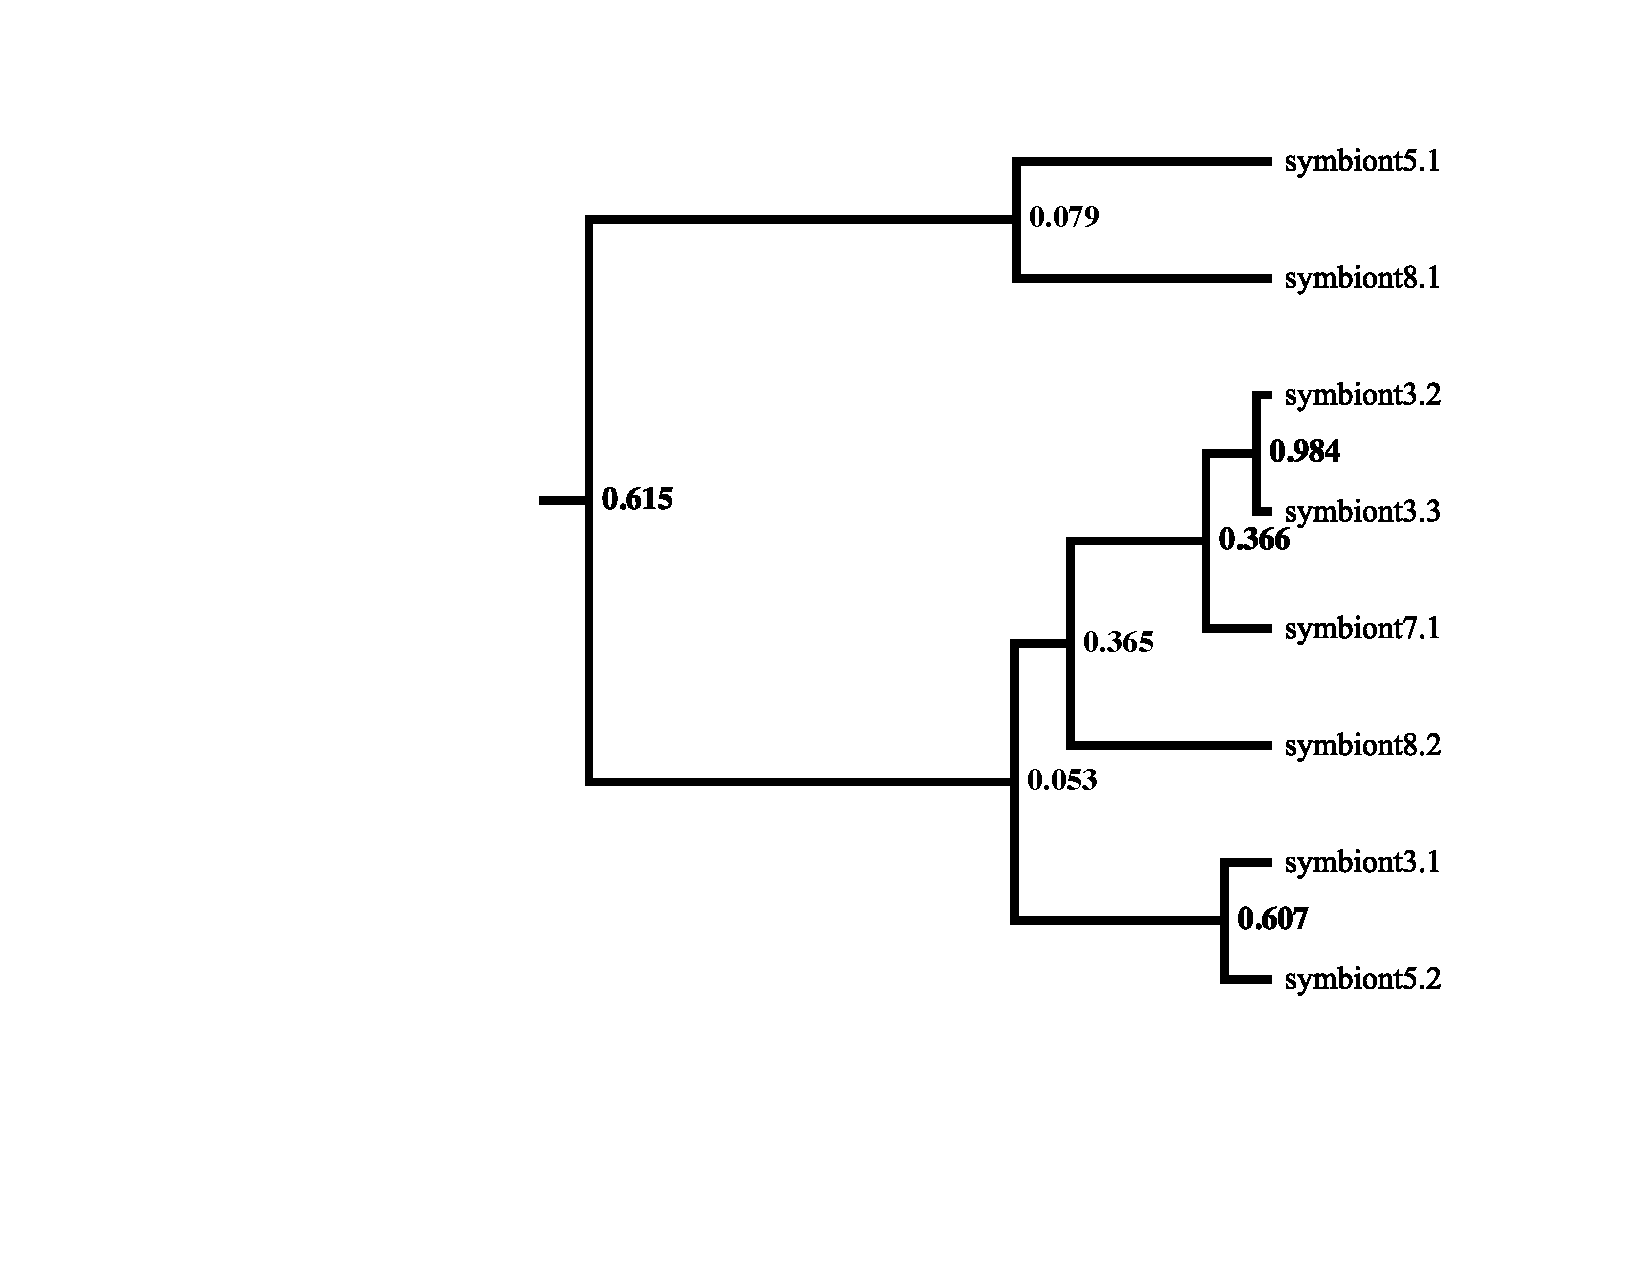
\includegraphics[width=0.66\textwidth]{figures/sim1.pdf}
\caption{The \ac{MCC} tree recovered from the }
\label{fig:sim1}
\end{SCfigure}

\begin{SCfigure}[0.66]
\centering
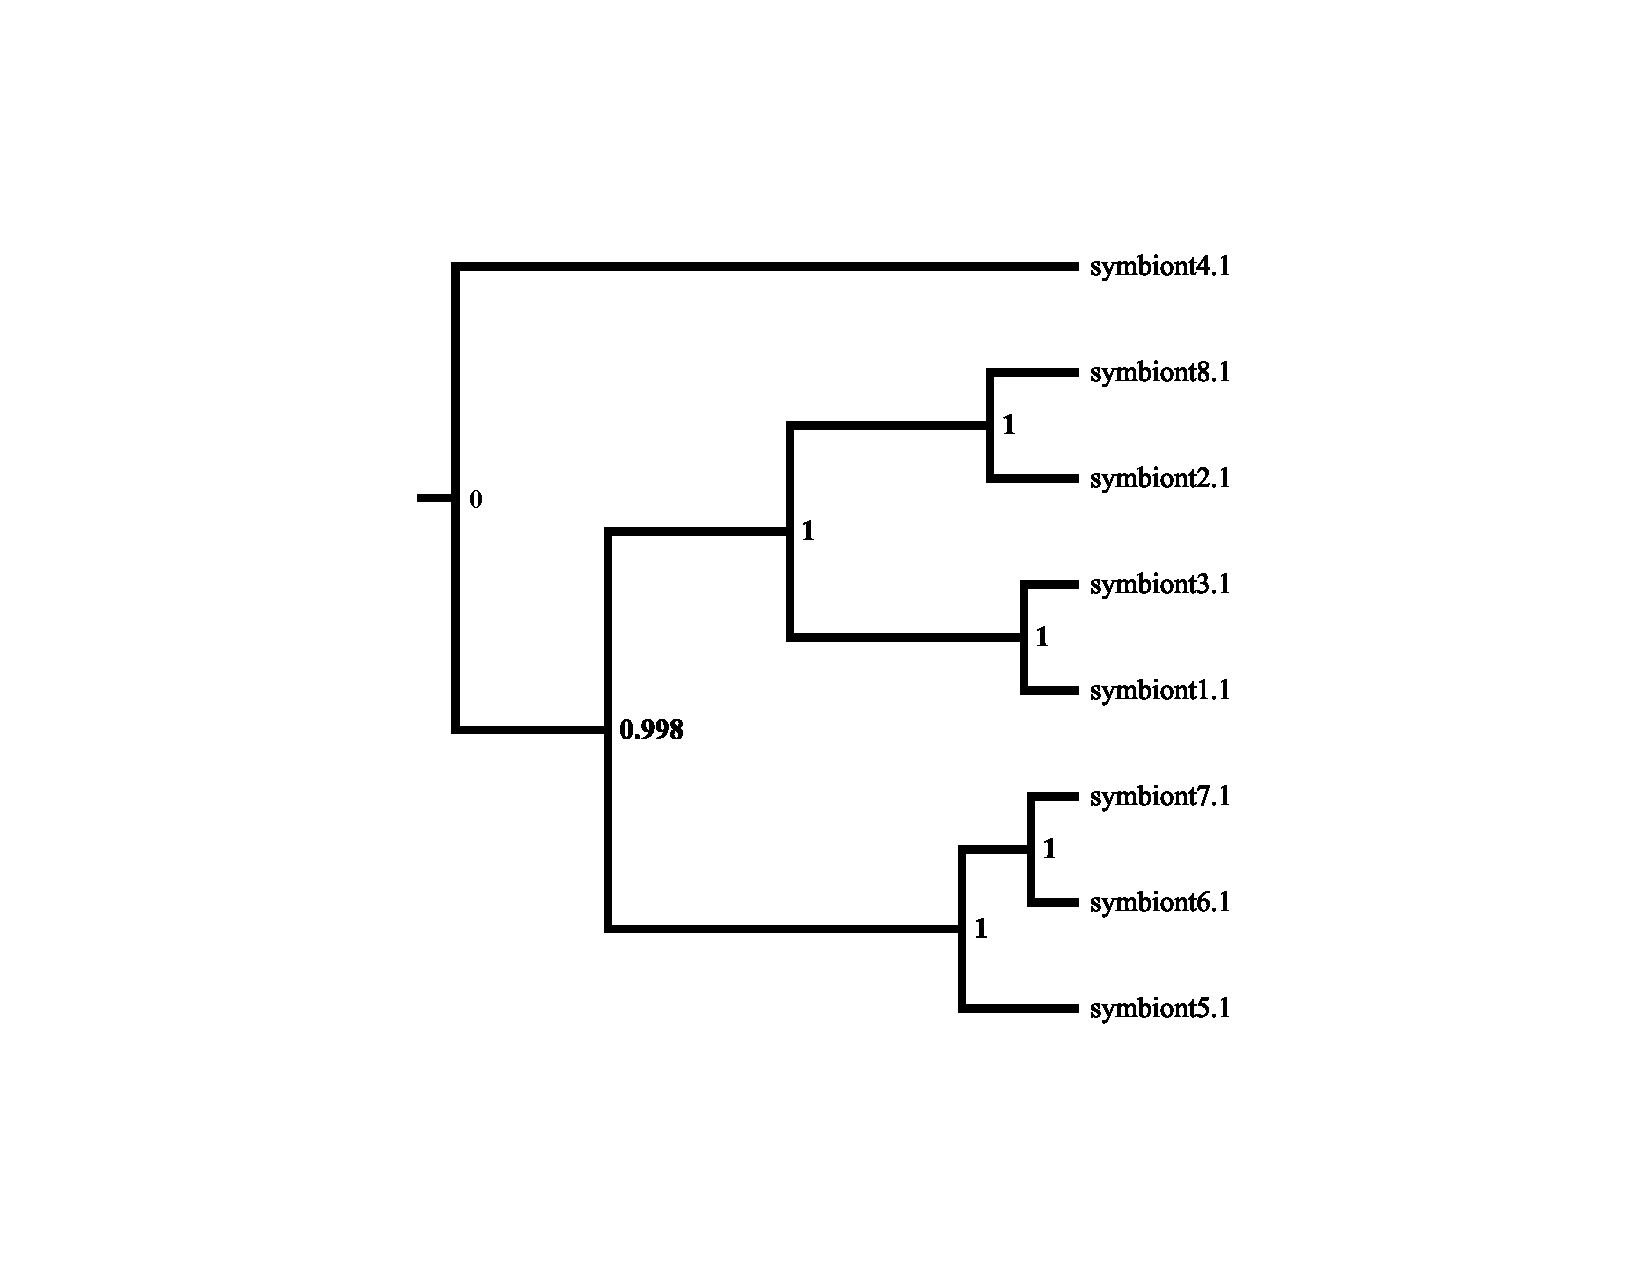
\includegraphics[width=0.66\textwidth]{figures/sim2.pdf}
\caption{The \ac{MCC} tree recovered from the }
\label{fig:sim1}
\end{SCfigure}


\section*{Discussion}

My cophylogeny reconstruction algorithm failed to recover 

\section*{Conclusions and Future Work}

I demonstrate a basic implementation of a simple cophylogeny model

An immediate problem is the inability for the and will necessitate . Along these lines, the effects of the cophylogeny likelihood on mixing of the \ac{MCMC} calls for serious investigation. 

At the time of writing, I have begun working with some real datasets, and . In addition to sequence data. Additionally

A significant effort has been put into developing and testing alternatives to the strict clock model for molecular evolution \parencites{Drummond:2006}{Drummond:2010}{Baele:2012b}, several of which have been implemented in BEAST and can be used with my cophylogeny model. Furthermore, in a model where rates can deviate, is the rate at a particular node better predicted by the symbiont or the host phylogeny? Testing these models against each other on real datasets can yield insight to these processes.

There are several avenues upon to expand the simple cophylogeny model. 

\textcite{Charleston:2002} and \textcite{Faria:2013} both found preferential host-switching to be a phenomenon 

I discussed . \textcite{Yang:2010} developed a Bayesian \ac{MCMC} methodology to determine the species delimitations between a set of individuals. Maintaining 

The model could also be expanded to support geographical data. In BEAST there are implementations of both discrete and continuous models for phylogeography \parencites{Lemey:2009}{Lemey:2010}, so a the location of a given symbiont node can be restricted to that of its host.

\ac{GMTC} . Ultimately, it may be possible , and thus to test the \ac{GMTC} against coevolutionary histories.

\printbibliography

\end{document}
